\section{RQ1: Where Does Per-Edit Validation Cost Go?}
\label{sec:rq1}

\paragraph*{Build and tests}
On networkx, the per-candidate build step (an editable install) takes a median of \NxBuildMedian\,s, \NxBuildShareTestsLo--\NxBuildShareTestsHi\pct{} of the serial test time.
The full suite of \NxNumTests{} tests passed at every state; serial test time per edit was \NxTestsLo--\NxTestsHi\,s across a first run and an idle re-run (median \NxTestsMedianClean\,s over the first run's clean-labelled states), of which about \NxPytestStartup\,s is pytest start-up and collection.
Over the base and the \NxReplayed{} replayed edits, serial tests alone took about \NxTestsSession\,s.

\paragraph*{Benchmarks}
One full benchmark pass (\NxBenchCases{} cases; our runner's cost protocol of two processes with three values each) took \NxBenchPassMin--\NxBenchPassMax\,s over \NxBenchPasses{} measured passes, with a median of about \NxBenchPassMedian\,s.
They are a dedicated pass at $S_0$, five unpatched sides of slowdown-oracle runs at later states, and three repeated passes at $S_0$ in one evening with machine telemetry, all with the same benchmark code and protocol; several were labelled noisy or concurrent.
Against about \NxBuildTests\,s for build plus serial tests, a benchmark pass costs at least about \NxBenchRatioTypical\x{} the rest of full validation even on the four fastest passes (\NxBenchPassMin--\NxBenchPassTypicalHi\,s), about \NxBenchRatioMedian\x{} at the median, and up to \NxBenchRatioHi\x{} (\NxBenchPassMax\,s) under drift, with the same code and protocol (Fig.~\ref{fig:cost}).
We lead with the lower bound because the claim is that benchmarks dominate, and because most passes were measured under load: by one uniform rule (a pass is noisy if any run exceeds the load gate or started without a passing gate), \PassesNoisy{} of the \NxBenchPasses{} passes are noisy, and the \PassesMeasured{} that is not is the unpatched side of an interleaved oracle run, so no pass is both clean and a dedicated full pass.
Pass times are run time only, excluding waits for the load gate.
The three repeated passes alone fell from \DriftEveningHi{} to \DriftEveningLo\,s (\DriftEveningRatio\x) within one evening, while their timing loops stayed at \DriftLoopsLo--\DriftLoopsHi\,s; almost all of the change was in one module's time outside the loops, and telemetry showed no covariate that moved with it.
Counting benchmarks, the build is below a fifth of a percent of a full validation at every measured pass.

\begin{figure}[t]
\centering
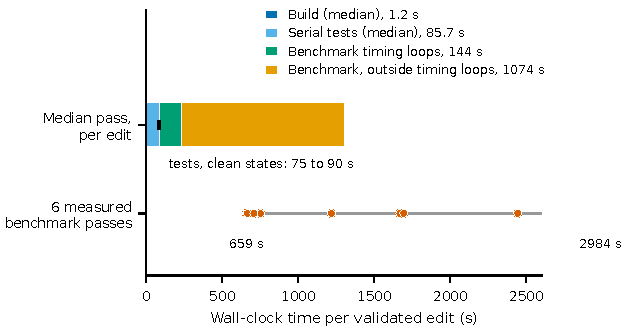
\includegraphics[width=\columnwidth]{figures/fig_cost.pdf}
\caption{Per-edit validation cost on networkx. Build and serial tests are medians with ranges over states; a full benchmark pass is split into time inside the timing loops and time outside them, over the measured passes (points). Single machine; wall times are ranges, not point values.}
\label{fig:cost}
\end{figure}

\paragraph*{Where benchmark time goes}
\NxAlgoShareLo--\NxAlgoShareHi\pct{} of a pass is spent in one module's \NxAlgoCases{} cases (\texttt{benchmark\_algorithms}), and \NxOutsideLoopsLo--\NxOutsideLoopsHi\pct{} of a pass lies outside the timing loops.
That module builds all its input graphs at import time, and asv's process isolation repeats the import for every case and process.
The timing loops themselves take only \NxLoopsLo--\NxLoopsHi\,s per pass.
If the setup were built once and reused, a pass would cost roughly its timing loops, about \NxSetupCachedLo--\NxSetupCachedHi\x{} build plus tests.
This is an estimate and a lower bound (it omits process start-up and warm-up), not a measurement.
\TODO{E5 (setup-cached pass): replace the estimate with a measured pass in which \texttt{benchmark\_algorithms}' graph construction moves into asv \texttt{setup\_cache} (or a cached fixture) in a patched copy of the suite; report loops, setup and total over at least three passes.}

Because the drift sits outside the timing loops, pass cost varies while verdicts on interleaved timed samples are shielded from slow drift (Appendix~\ref{app:drift}); it also means the setup, not the timing, is what a cached pass would remove.

\paragraph*{Contrast: a C extension}
On bottleneck, a clean build takes \BnBuildLo--\BnBuildHi\,s and the full suite (\BnNumTests{} tests) about \BnTests\,s, so the build is about \BnBuildShareLo--\BnBuildShareHi\pct{} of build plus tests.
Two full benchmark passes (\BnBenchCases{} cases, the same protocol, one state) took \BnBenchPassLo{} and \BnBenchPassHi\,s, so benchmarks cost about \BnBenchRatioLo--\BnBenchRatioHi\x{} build plus tests here too, and the build falls to about \BnBuildShareBenchLo--\BnBuildShareBenchHi\pct{} of a full validation.
Unlike networkx, the two passes agree closely, and about \BnLoopsShare\pct{} of the benchmark time is in the timing loops; we did not decompose the rest.
All bottleneck runs were labelled noisy, and the result covers one state.
\TODO{E4: R1 on one replication project with a cheap build and an asv suite (build, full tests, full benchmarks at 3--5 states, three passes each).}

\paragraph*{Answer to RQ1}
On networkx, benchmarks dominate per-edit validation cost, at least about \NxBenchRatioTypical\x{} build plus tests even on the fastest passes (about \NxBenchRatioMedian\x{} at the median), and most of their time lies outside the timing loops in one module, largely import-time setup by inspection; with that setup cached, the estimate drops to \NxSetupCachedLo--\NxSetupCachedHi\x, still the largest part but not by an order of magnitude.
Reducing the build saves almost nothing for this pure-Python project; reducing tests saves at most the test time of about a minute and a half per edit.
On bottleneck, a C-extension project with a non-trivial build, benchmarks also dominate, at about \BnBenchRatioLo--\BnBenchRatioHi\x{} build plus tests at one state.
